\documentclass{beamer}

\mode<presentation>
{
\usetheme{Warsaw}

\setbeamercovered{transparent}
}

\usepackage[english]{babel}
\usepackage[latin1]{inputenc}
\usepackage{listings}
% font definitions, try \usepackage{ae} instead of the following
% three lines if you don't like this look
\usepackage{mathptmx}
\usepackage[scaled=.90]{helvet}
\usepackage{courier}

\setbeamertemplate{footline}[frame number]


\usepackage[T1]{fontenc}

\lstset{language=Python, numberstyle=\tiny, keywordstyle=\color{blue},numbers=left,commentstyle=\color{green},
basicstyle=\footnotesize}


\title{The architecture of robotics control software for heterogeneous mobile
robots network}


\author {Kirsanov Kirill\inst{1} \inst{2}}


\institute
{
\inst{1}
Laboratory "Sensorika", Miusskaya sq., 4, 125047, Moscow, Russia
\and
\inst{2}
Moscow state technological University 'Stankin', Vadkovsky per. 3a, 101472,
Moscow, Russia

}
\date{2013.10.25 // DAAAM International Symposium}
\beamerdefaultoverlayspecification{<+->}
\begin{document}
\begin{frame}
\titlepage
\end{frame}

\section{Introduction}
\begin{frame}
\frametitle{3 levels of control for robot}
There are 3 levels of abstractions to control robot
\begin{itemize}
	\item<1>{\textbf{Hardware} - Voltage, current, pressure etc.} 
	\item<1>{\textbf{Software} - Programs in programming language -
	C/C#/java/assembler/verilog etc.}
	\item<1>{\textbf{AI-ware} High level cognetive commands, like ''walk'',
	''weld'', even ''make jobs done''}
\end{itemize}
\textbf{This work is specially dedicated for software level}
\end{frame}


\subsubsection{Robotics Software}
\begin{frame}
\frametitle{Robotics Software}
\framsubetitle{Robotics Development Kits:}
There are many types of robotic software
\begin{itemize}
\item<1> \textbf{ROS robotic Operating System}
\item<1> \textbf{Microsoft Robotics Studio} 
\item<1> \textbf{Player Project} 
\item<1> \textbf{ORCA2} 
\item<1> \textbf{LAAS/GenoM} 
\item<1> \textbf{Marie} 
\item<1> \textbf{URBI} 
\item<1> \textbf{Webots} 
\item<1> \textbf{RoboJRE}
\item<1> \textbf{OROCOS}
\item<1> \textbf{Software Development Kits for specific robots like Festo, ABB,
Kuka etc..}
\end{itemize}
\end{frame}

\begin{frame}
\frametitle{Destination of Robotics Software}
\begin{itemize}
\item Destination of Robotics Software - hide the complexity of the real
world of abstractions.
\item Last 10 years abstractions fully hide the robot from developer.
\end{itemize}
\end{frame}


\subsection{Software as a tool for robotics}
\begin{frame}
\frametitle{Computer as a tool for robotics}
\framesubtitle{Factorial example}
Software from previous slide is only a tool for developer. But this tool have a
strong influence on way of thinking:
\begin{itemize}
  \item<1> Mathematics: Factiroal by the recurrence relation: \\
  	\large $F(x) = {\{^{1 | x=0}_{F(x-1)*x | x>1}}$
  \item<1> C++: Factiroal by the recursive function	
		\lstinputlisting[language=C]{fac.c} 
  \item<1> Haskell. Easy way
        \lstinputlisting[language=Haskell]{face.hs}  
\end{itemize}
\normalsize
\end{frame}

\begin{frame}
\frametitle{Software as a tool for robotics}
\framesubtitle{Factorial example. Continue.}

\begin{itemize}
  \item<1> Python: Factiroal by the reduction:
	\lstinputlisting{fac.py}
  \item<1> Assembler: Factiroal by byte operations
		\lstinputlisting[language=C]{fac.asm}   
\end{itemize}
\end{frame}

\begin{frame}
\frametitle{Software as a tool for robotics}
\framesubtitle{Factorial example. End.}
\begin{itemize}
  \item<1> Haskell. Combinatory reduction
		\lstinputlisting[language=Haskell]{fac.hs}
\end{itemize}

There are another haskell example with explicit type recursion, 
functors, comonads, generalized catamorphisms,
zygomorphisms and paramorphisms. \\ See
www.willamette.edu/~fruehr/haskell/evolution.html
\end{frame}


\subsection{Complicated software}
\subsubsection{complex vs. simple}
\begin{frame}
\frametitle{Complicated software}
\begin{itemize}
  \item<1> {Modern robotics software from previous slide are very complex and
  complicated.}
  \item<1> {To use this software properly you need to be a high level
  programmer.}
  \item<1> {If you have a problem with control, and want to use new foftware to
  overcome it - then you have two problems}
  \item<1> {In R\&D the are many new tasks which one are not covered by
  software}
  \item<1> {There are many proprietary devices are not supported by common
  robotics software}
\end{itemize}
\end{frame}

\section{Our approach}
\subsection{Simple is better than complex}
\begin{frame}
\frametitle{Our approach - Simple is better than complex}
\framesubtitle{Complex is better than complicated}
Network
\begin{itemize}
  \item<1> Fully connected network of nodes instead of complex graphs
  \item<1> Stay close to TCP/IP stack as possible - no need in special
  protocols. Only simple JSON encoded dynamic-typed messages.
\end{itemize}

Programming
\begin{itemize}
  \item<1> Give a possibility to avoid any special library or
  framework.
  \item<1> No need in special file structure, compiler or translator.
\end{itemize}

Language
\begin{itemize}
  \item Strict dynamic typed interpreted language are prefered.
\end{itemize}
\end{frame}

\subsection{Virtual IO}
\begin{frame}
\frametitle{Virtual IO}
\framesubtitle{No frivers for common software}
\framesubtitle{Robot example 1 - Sensorika}
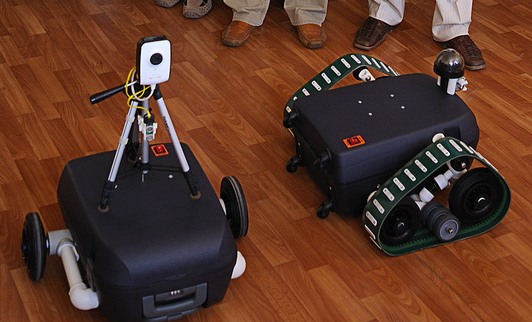
\includegraphics[width=9.5cm]{rob1.jpg}
\end{frame}

\begin{frame}
\frametitle{Virtual IO}
\framesubtitle{No frivers for common software}
\framesubtitle{Robot example 2 - BROKK}
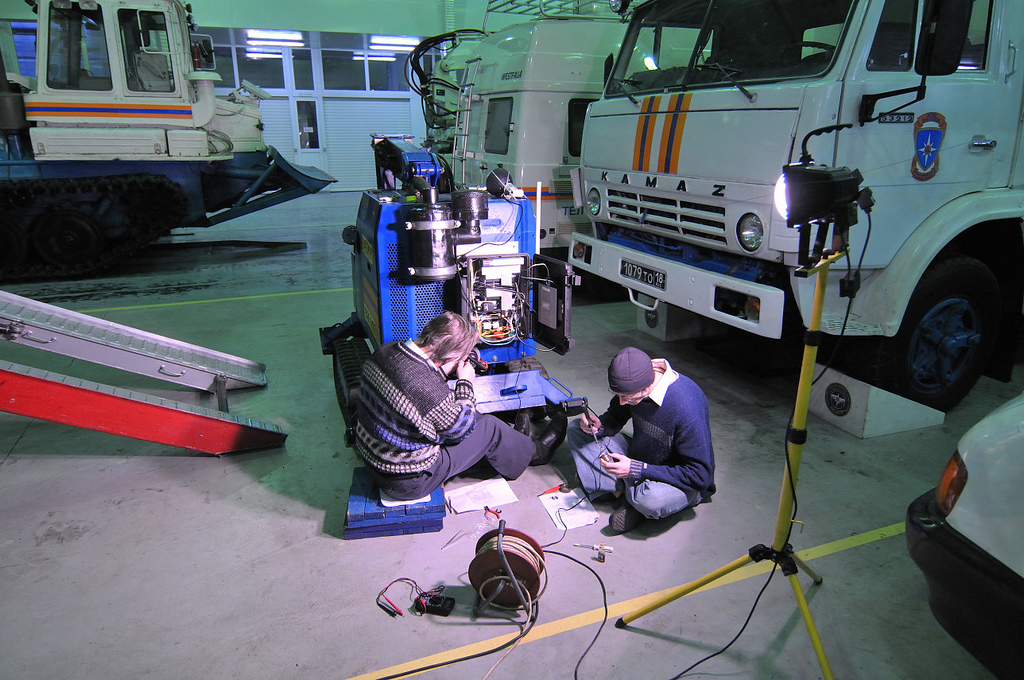
\includegraphics[width=9.5cm]{robot_big.jpg}
\end{frame}

\begin{frame}
\frametitle{Virtual IO}
\framesubtitle{Drivers for ROS are avaliable}
\framesubtitle{Robot example 3 - Robotino-Robotio XT}
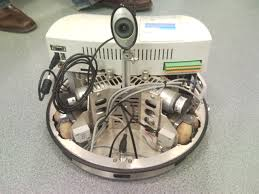
\includegraphics[width=7.5cm]{robotino.jpg}
\end{frame}

\begin{frame}
\frametitle{Virtual IO} 
\begin{itemize}
  \item<1> There are many types of IO ports: CAN, COM, USB etc.
  \item<1> Robotics software requires uniform access and guarantee it with
  special drivers for each port and device
  \item<1> There are so many mechatronic devices. It is often not possible to
  provide a uniform access method to all mechatronic devices.
  \item<1> What should we do, if we have to incorporate some robot or device in
  our network, but there are only proprietary softoware for it? \alert{IO ports
  virtualization}
\end{itemize} 
\end{frame}


\begin{frame}
\frametitle{Virtual IO} 
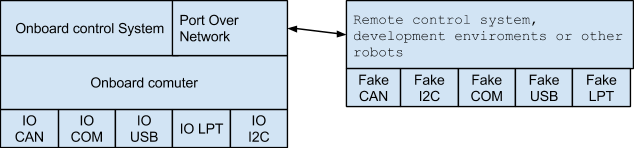
\includegraphics[width=8.5cm]{io.png}
\begin{itemize}
  \item<1> 
     In this case, "mirrors" of input/output ports are programmatically created
     on the remote computer (such as the developers computer) with the same features and timeouts.
  \item<1>      
     This allows you to use proprietary control software without any networking intention, or to easily integrate it into your own designs.
\end{itemize}

\end{frame}

\subsection{Developing software}

\subsection{How does they work?}
\begin{frame}
\frametitle{How does they work?}
\begin{itemize}
	\item<1>Main development language: C, Java, C\# etc.
	\item<1>'Multi-agent approach' (System are composed of multiple interacting agents like engine, sensor, camera, etc.).
	\item<1>This agents interacts via RPC (Remote Procedure Call) abstraction.
\end{itemize}
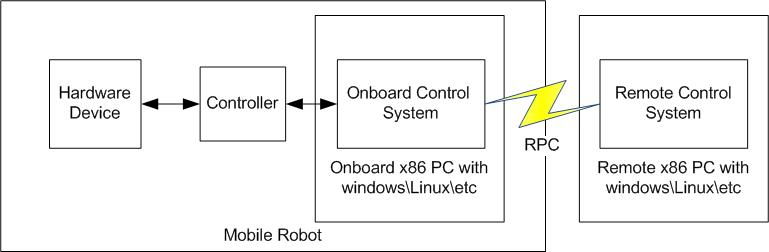
\includegraphics[width=10.5cm]{rpc0.jpg}
\end{frame}


\begin{frame}
\frametitle{Real robot != model}
\begin{itemize}
\item<1>RPC implies a call for existing functions, while the development process is accompanied by their creation and
modification. Thus, there is need for continuous updating the interprocess communication protocol and on-board control 
system.
\item<1>Onboard control system implemented on a compiled language, and any update requires them to be re-compiled and
restarted;
\end{itemize}
Disadvantages: 
\begin{itemize}
\item<1>It`s hard to develop - creating and testing of new algorithms requires a fairly lengthy restart procedure 
 and greatly slows development process;
\item<1>It`s hard to debug - impossible to dynamicly update working code onboard;
\end{itemize}
\end{frame}

\subsection{New system arcitecture}
\begin{frame}
\frametitle{New system arcitecture}
\framesubtitle{Not just another RDK or framework but new paradigm}

To overcome this difficulties we are using:
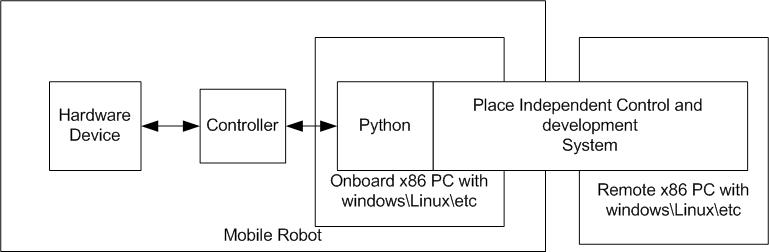
\includegraphics[width=10.5cm]{rpc1.jpg}
\begin{itemize}
 \item<1>A dynamic interpreted language Python as a base testing and development language;
 \item<1>Implemented Turing-complete protocol;
\end{itemize}
\end{frame}


\section*{Summary}

\begin{frame}
\frametitle<presentation>{Summary}

\begin{itemize}
  \item<1> Modern robotics software are very complicated. In some fields such
  R\&D it`s easier to withdraw it
  \item<1> Ours approach is good for us in some tasks of R\&D in industry and
  science.
\end{itemize}

\vskip0pt plus.5fill

\begin{itemize}
  \item<1> In future, where there is no driver-related problems, our approach
  will migrate into ROS or other robotics software as a middleware.
\end{itemize}
\end{frame}


\begin{frame}
      \begin{center}
        \font\endfont = cmss10 at 25.40mm
        \endfont 
        \baselineskip 20.0mm
        Thank you
      \end{center}    
\end{frame}

\end{document}
